\documentclass{article}
\usepackage[left=0.25in, right=0.25in, top=0.05in, bottom=0.05in]{geometry}
\usepackage{tikz,pgfplots, graphicx,subfigure}

\begin{document}
	\begin{center}
		Convergence of interpolation using Uniform nodes and Chebyshev nodes\\
		{\Huge $$\exp(-\left\vert x \right\vert)$$}
	\end{center}

	\begin{figure}[!htbp]
		\begin{center}
		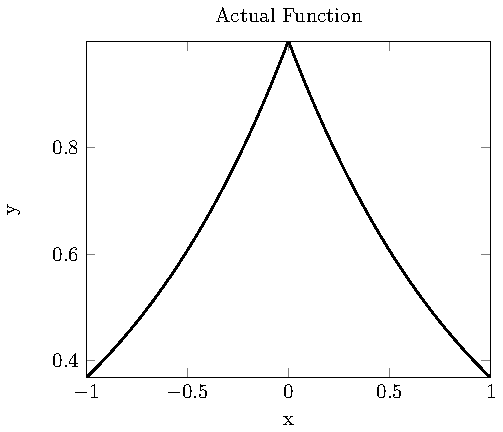
\includegraphics[scale=2.25]{./Actual_Function.pdf}
		\caption{Actual function}
		\end{center}
	\end{figure}
	\begin{figure}[!htbp]
		\begin{center}
		\subfigure[5 nodes]{
			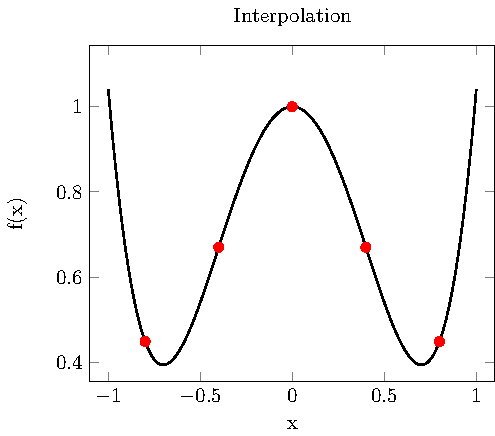
\includegraphics[scale=0.8]{./Uniform_interpolant_5.pdf}
		}
		\subfigure[10 nodes]{
			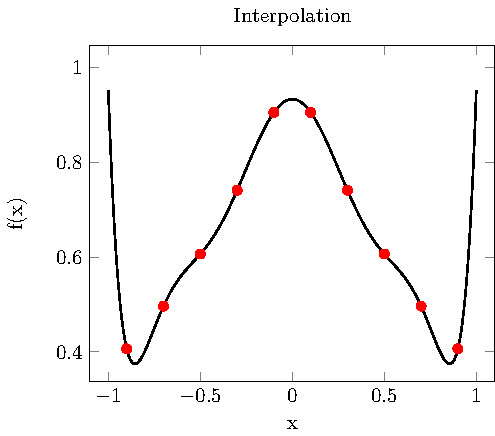
\includegraphics[scale=0.8]{./Uniform_interpolant_10.pdf}
		}
		\subfigure[20 nodes]{
			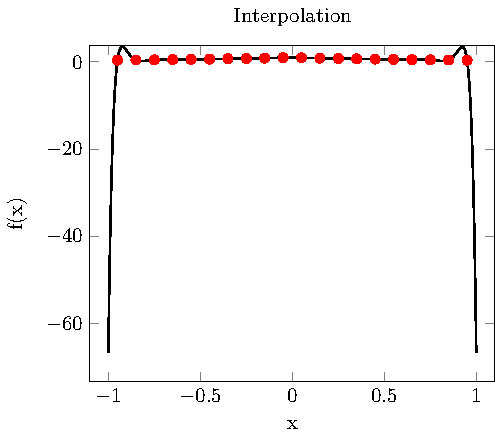
\includegraphics[scale=0.8]{./Uniform_interpolant_20.pdf}
		}
		\subfigure[40 nodes]{
			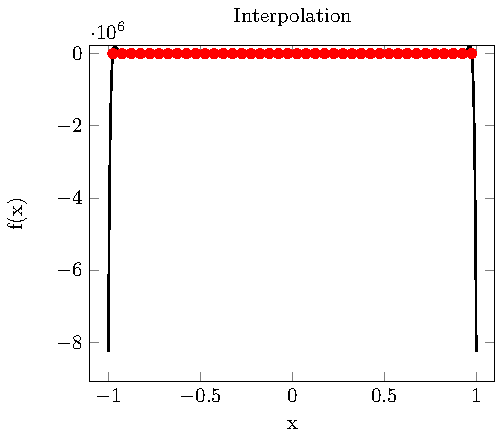
\includegraphics[scale=0.8]{./Uniform_interpolant_40.pdf}
		}

		\subfigure[80 nodes]{
			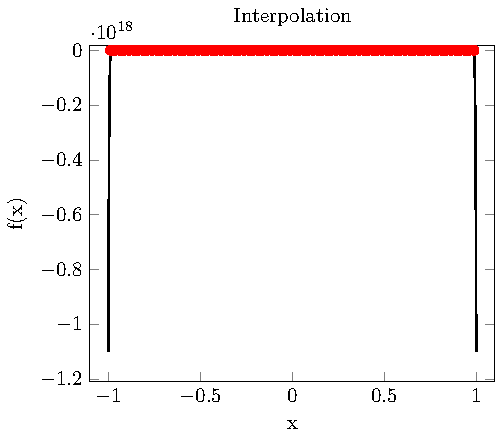
\includegraphics[scale=0.8]{./Uniform_interpolant_80.pdf}
		}
		\subfigure[160 nodes]{
			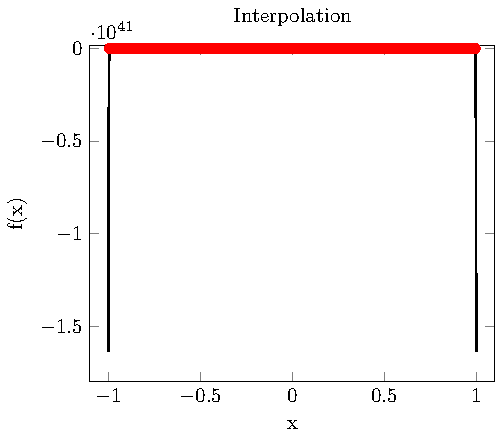
\includegraphics[scale=0.8]{./Uniform_interpolant_160.pdf}
		}
		\subfigure[320 nodes]{
			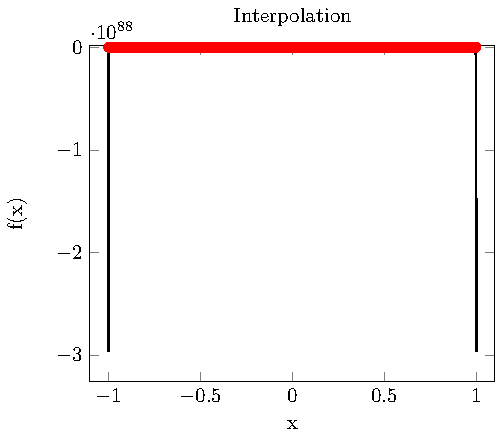
\includegraphics[scale=0.8]{./Uniform_interpolant_320.pdf}
		}
		\subfigure[640 nodes]{
			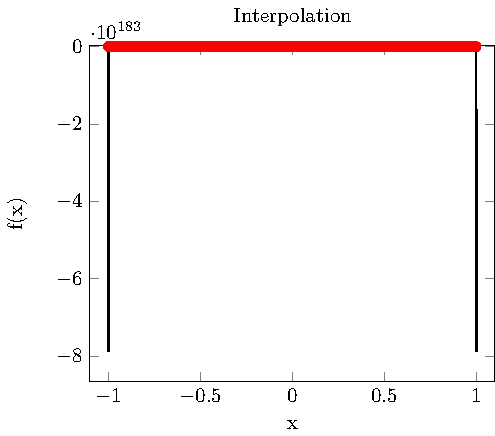
\includegraphics[scale=0.8]{./Uniform_interpolant_640.pdf}
		}
		\caption{Chebyshev interpolation}
		\end{center}
	\end{figure}
	\begin{figure}[!htbp]
		\begin{center}
		\subfigure[5 nodes]{
			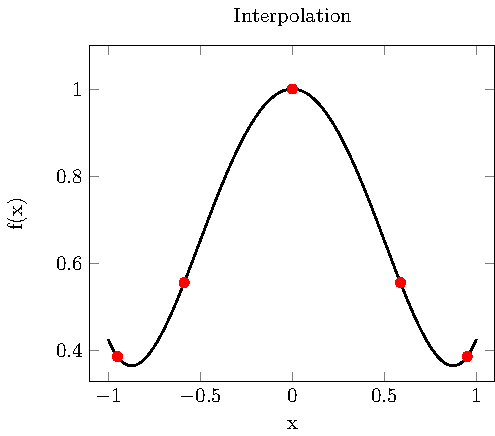
\includegraphics[scale=0.8]{./Cheb_interpolant_5.pdf}
		}
		\subfigure[10 nodes]{
			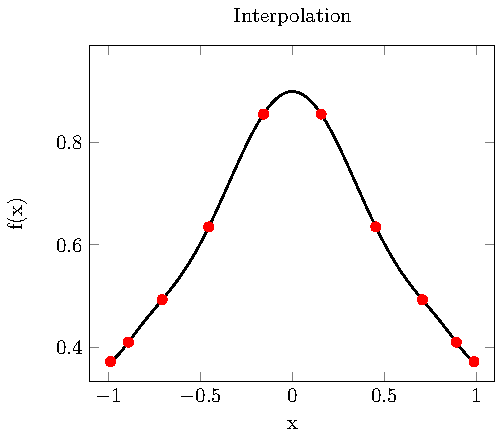
\includegraphics[scale=0.8]{./Cheb_interpolant_10.pdf}
		}
		\subfigure[20 nodes]{
			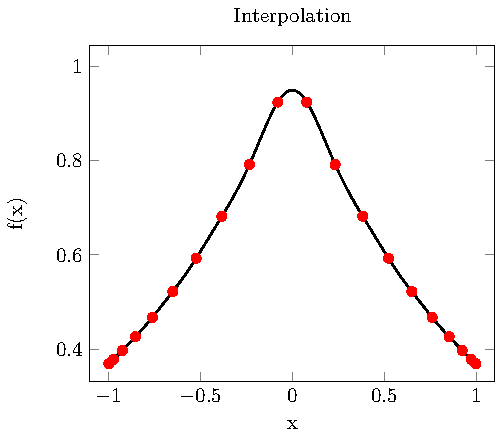
\includegraphics[scale=0.8]{./Cheb_interpolant_20.pdf}
		}
		\subfigure[40 nodes]{
			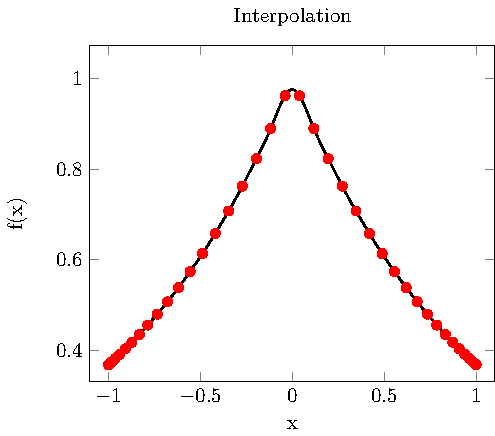
\includegraphics[scale=0.8]{./Cheb_interpolant_40.pdf}
		}

		\subfigure[80 nodes]{
			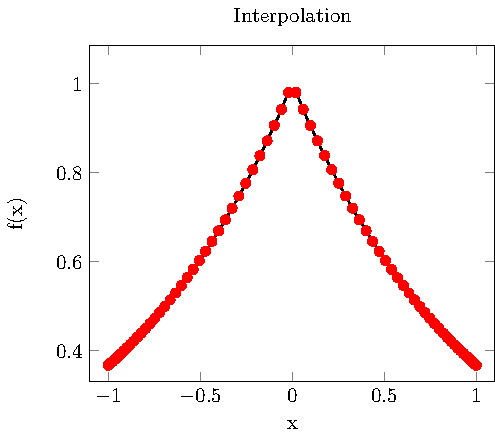
\includegraphics[scale=0.8]{./Cheb_interpolant_80.pdf}
		}
		\subfigure[160 nodes]{
			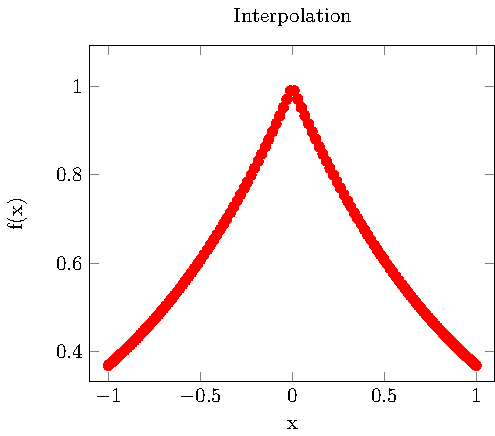
\includegraphics[scale=0.8]{./Cheb_interpolant_160.pdf}
		}
		\subfigure[320 nodes]{
			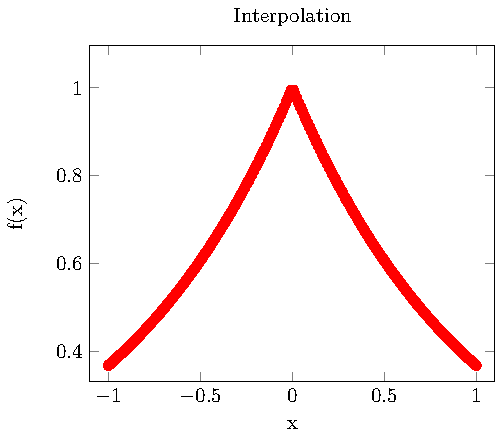
\includegraphics[scale=0.8]{./Cheb_interpolant_320.pdf}
		}
		\subfigure[640 nodes]{
			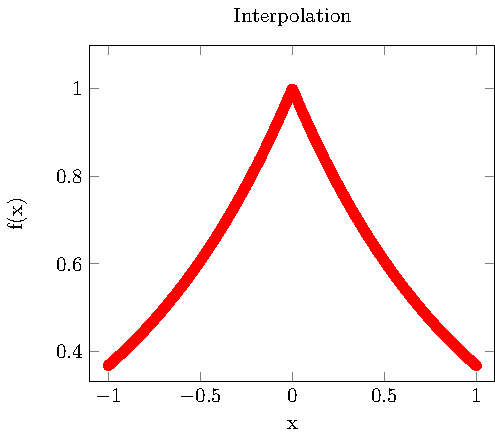
\includegraphics[scale=0.8]{./Cheb_interpolant_640.pdf}
		}
		\caption{Chebyshev interpolation}
		\end{center}
	\end{figure}
\end{document}